\section{Challenges of the conventional analysis methods}
In this section, I will briefly introduce the conventional analysis methods used in the field, two fundamental challenges faced with the current method, and discuss the existing approaches to address these challenges and their limitations. 

%todo: make changes to clarify the things I want to say with the grant claims.
Fundamentally, experimental results capture the interaction between the probe and the target. To distill the scientific essence presented in the results, complex analysis is usually required. In the case of microscopy measurements like STM, conventional methods like \ac{FT} are commonly used \cite{ardiniHighthroughputMultimodalWidefield2023}\cite{jaffeDifferenceFourierAnalysis1987}
\noindent \cite{sciuttoFTNIRMicroscopyAdvanced2014}\cite{kimotoAssessmentLowervoltageTEM2012}. The \ac{FT} reveals characteristic wavelengths and provides insights to the underlying scientific theories of the specimen studied. This is particularly true in cases where the microscopy results contain near perfect periodic features, but when aperiodic signals are presented, the \ac{FT} is less ideal and suffers from loss of information. 

There are 2 specific challenges in QPI analysis with the conventional \ac{FT} method we would like to focus on, the speckle problem and the demixing problem. We will also establish their mathematical formulations, which will lead to the convolutional data model we present later. 

Fundamentally, the data obtained from experiments—particularly in techniques like quasiparticle interference scanning tunneling microscopy (QPI-STM)—are not direct representations of the underlying physical mechanisms. Instead, they are convolutions of the interpretable signatures we aim to extract (such as interference patterns or defect-induced modulations) with a range of additional contributions—instrument response, scanning junction variations, and noise. This complexity means that careful data analysis is often essential to uncover the true physical insights. Among conventional methods, the Fourier Transform (FT) is widely used to extract characteristic wavelengths and relate them to theoretical predictions across different systems \cite{ardiniHighthroughputMultimodalWidefield2023}\cite{jaffeDifferenceFourierAnalysis1987}
\noindent \cite{sciuttoFTNIRMicroscopyAdvanced2014}\cite{kimotoAssessmentLowervoltageTEM2012}.

However, FT has notable limitations, especially when applied to more complex or less ideal datasets. In systems with nearly perfect periodicity, FT produces sharp, interpretable peaks. But in more realistic scenarios—where signals include aperiodic features such as randomly distributed defects —the FT tends to produce blurred spectra, diffuse speckles, and loss of phase information. This can severely hinder the interpretability of the results and mask the very features researchers are trying to study. While these challenges are particularly evident in QPI-STM, similar issues arise in other imaging and spectroscopic techniques where signal complexity or disorder is present\cite{Bonnet 1997} \cite{Draijer 2009}.

In the context of QPI analysis, these limitations give rise to two specific and critical problems we aim to address: the speckle problem and the demixing problem. In the following, we will define these challenges more formally and introduce a convolution-based data model designed to overcome them.
\begin{figure}
	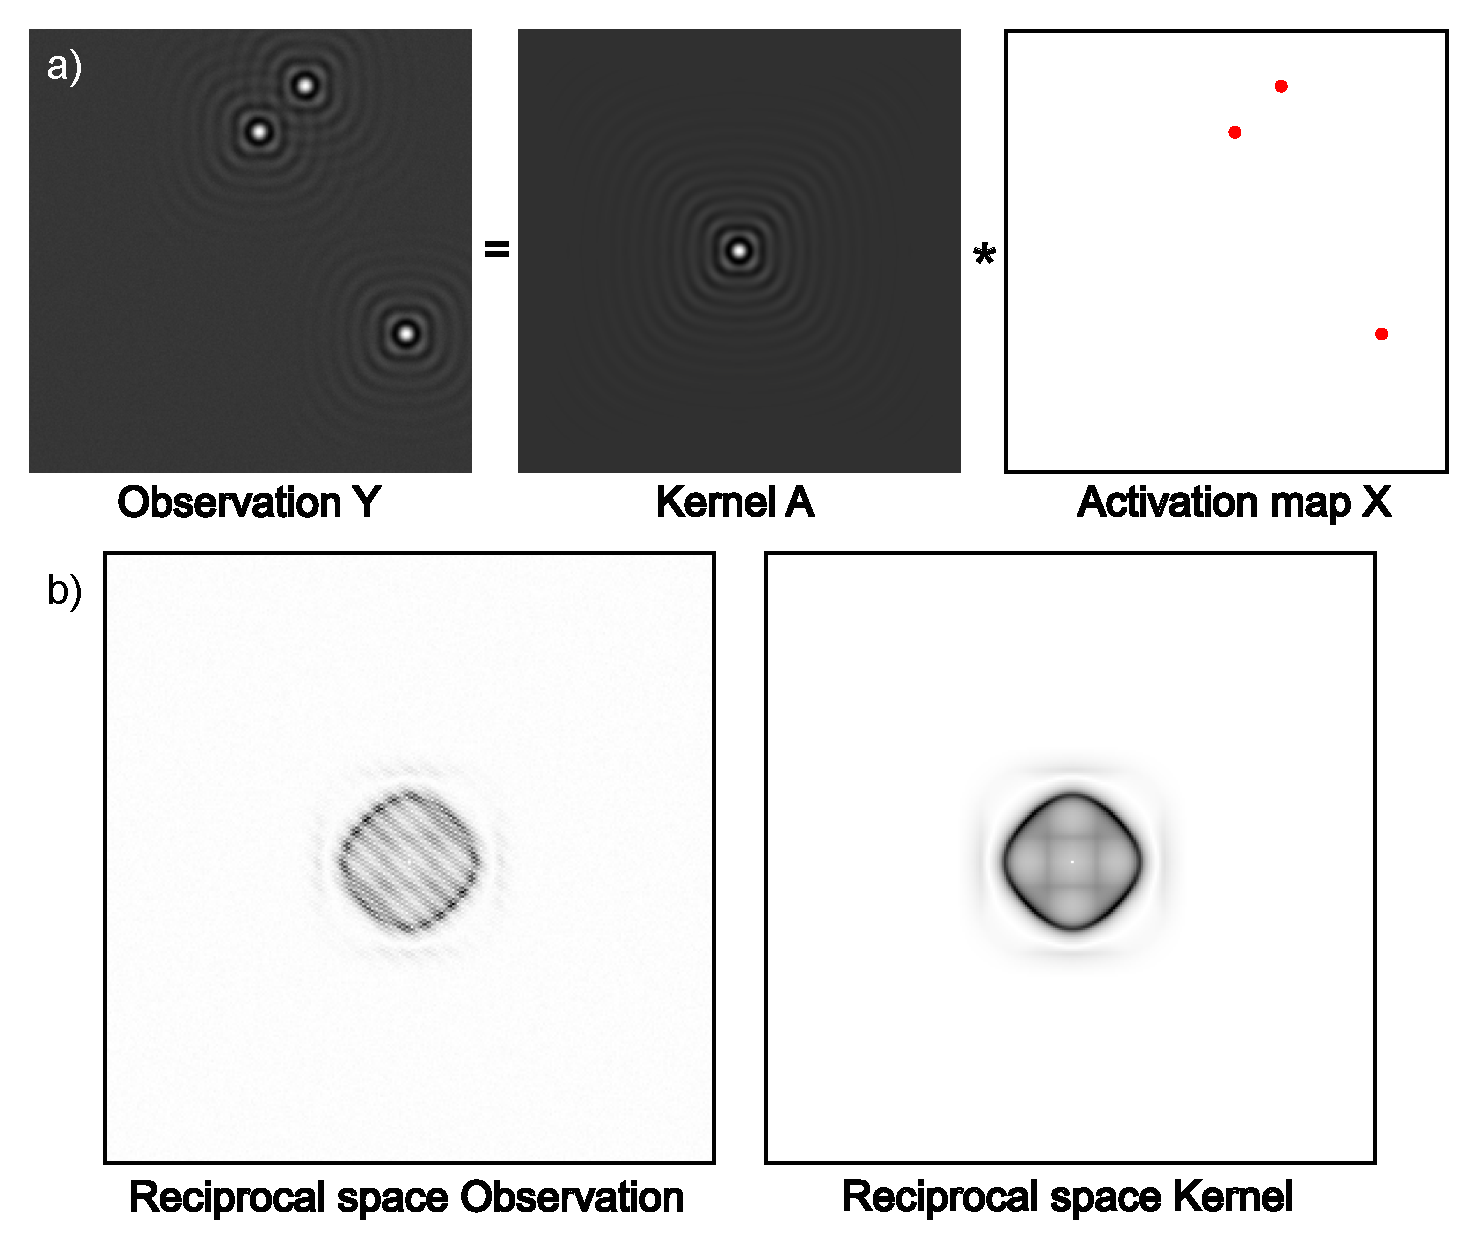
\includegraphics[width= \textwidth]{Ch6_deconvolution.pdf} 
	\centering
	\caption{Illustration of the observation generation process and the speckle problem. a) The QPI-STM data generation process can be seen as the convolution between the QPI pattern of a defect (the kernel A) and its location map (the activation map X). We can take the Fourier transform of the observation and the kernel, respectively and get b); clear speckle is presented in the FT-observation, which hindered the desired pattern of $\delta\rho_0$ as presented on the right}
	\label{fig:ch6_decon}
\end{figure}

\subsection{The Speckle problem}
As introduced in the end of Ch5 and theorized explicitly in Equation \ref{eq.539}, when we take \ac{FT} of the grid map on multiple occurrence of defects, we get speckle on the \ac{FT-STS}. The problem is that the spatial distribution information of the defect location manifest as undesirable patterns in the \ac{FT} space, and makes the QPI pattern hard to interpret. Therefore, to address the challenge of speckle is to disentangle the spatial information from the \ac{QPI} pattern, and this can be formulated mathematically as a deconvolution problem. 

\par \noindent Recall that we can write the modulation of \ac{LDOS} $\delta \rho$ from multiple defects as:
\begin{equation}
	\delta \rho(\mathbf{x}, \omega) = \sum_{j=1}^{N}c_j \cdot \delta \rho_0(\mathbf{x}-\mathbf{x_j},\omega),
\end{equation}
\noindent where $\delta \rho_0$ is the \ac{LDOS} modulation from individual defect located at at $\mathbf{x_j}$. We can further separate the spatial information by utilizing a Kronecker delta $\Delta(\mathbf{u})$, so that $\Delta(\mathbf{u})=1$ if $\mathbf{u} = 0$, and $\Delta(\mathbf{u})=0$ elsewhere: 
\begin{equation}
	\sum_{j=1}^{N}c_j \cdot \delta \rho_0(\mathbf{x}-\mathbf{x_j},\omega) = \sum_{\mathbf{u}} \delta \rho_0(\mathbf{x}-\mathbf{u},\omega)\cdot(\sum_{j=1}^{N} c_j \cdot \Delta(\mathbf{u-x_j})).
\end{equation}
\noindent We can then construct a convolution sum between the individual \ac{QPI} pattern and the spatial information by defining a defect location function $D(\mathbf{x}) \equiv \sum_{j=1}^{N} c_j \cdot \Delta(\mathbf{u-x_j})$, we have: 
\begin{equation}
	\delta \rho(\mathbf{x}, \omega) =  \sum_{\mathbf{u}} \delta \rho_0(\mathbf{x}-\mathbf{u},\omega)\cdot D(\mathbf{u}) = (\delta \rho_0 *D)(\mathbf{x}, \omega).
\end{equation}

We illustrate this convolution in Fig. \ref{fig:ch6_decon} a); first, we use $\delta \rho_0$ simulated in Ch.5.2 as the \ac{QPI} pattern from an single defect, we then randomly generate a binary defect location map given a defect density, and use the convolution sum to construct an observation. To unify the language, we will now refer to the single defect \ac{QPI} pattern as a kernel, denoted as A, and the defect location map as an activation map, denoted as X; thus, we can express our observation as $Y = A * X$. Then, we follow the conventional approach and take \ac{FT} of both the observation Y and the kernel A As shown in panel b), the \ac{FT} of Y shows clear speckle compared to the \ac{FT} of the kernel.

There have been few attempts made to address the speckle, partially because speckle are less disruptive at higher defect density, as illustrated in the Figure. \ref{fig:ch5_changephasenoise}. Another "mitigation" is through brute force and finding an isolated defect, which is possible in low defect concentration materials but less so with dense defects. Recently, due to advancement in machine learning, researchers treated speckle as a source of noise and try to address it with self-supervised algorithms like Noise2Self \cite{kuijfSelfsupervisedLearningDenoising2025}, this present good performance in synthetic data, however, the blackbox nature of the machine learning algorithm makes it hard to tell the performance in real data, as the denoising process is hard to interpret. Another line of effort is the development of deconvolution algorithms, which includes the SBD-STM algorithm presented by Cheung et al \cite{cheungDictionaryLearningFouriertransform2020}, which inspired this body of work.
 

\subsection{The Demixing problem}
%todo: how should I include the general motivation of demxing? or is it enough here? 
Materials normally exhibit multiple types of defects, and these defects could present different scattering features. Many QPI measurements have exploited the mechanisms of selectivity scattering channels across a wide variety of materials, such as the sign variation of the superconducting order parameter \cite{chiSignInversionSuperconducting2014}, the spin and orbital texture of topological bands \cite{yinProbingTopologicalQuantum2021}\cite{butlerQuasiparticleInterferenceZrSiS2017}. 

To access impurity-dependent scattering information requires demixing different defects from a single grid map. However, there are only limited approaches to analyze and disentangle defect-dependent scattering features. The most common approach is to acquire grid spectroscopy on isolated defects, or to crop around individual defects in larger grid maps if the isolated defect is hard to find. One example is the Dirac semimetal ZrSiS, where the interference patterns around impurities located on the Zr and S sublattice sites scatter differently \cite{butlerQuasiparticleInterferenceZrSiS2017}; As shown in Figure. \ref{fig:ch6_ZrSiS}, conventional \ac{FT} displays a mixture of the scattering features, which are disentangled through inspecting the \ac{FT} of cropped grid spectroscopy around individual defects. 

There are 2 primary shortcomings with this approach: one is due to a small spatial range of the cropping, the resolution in q-space is very much limited, making it hard to resolve features with higher frequencies. Second is that the cropped area could still preserve features from other defect sources, this is particularly problematic when we have quasiparticles with longer lifetime; The long decaying tail could easily spread tens or hundreds of unit cells, making it hard to avoid when cropping. 

\begin{figure}
	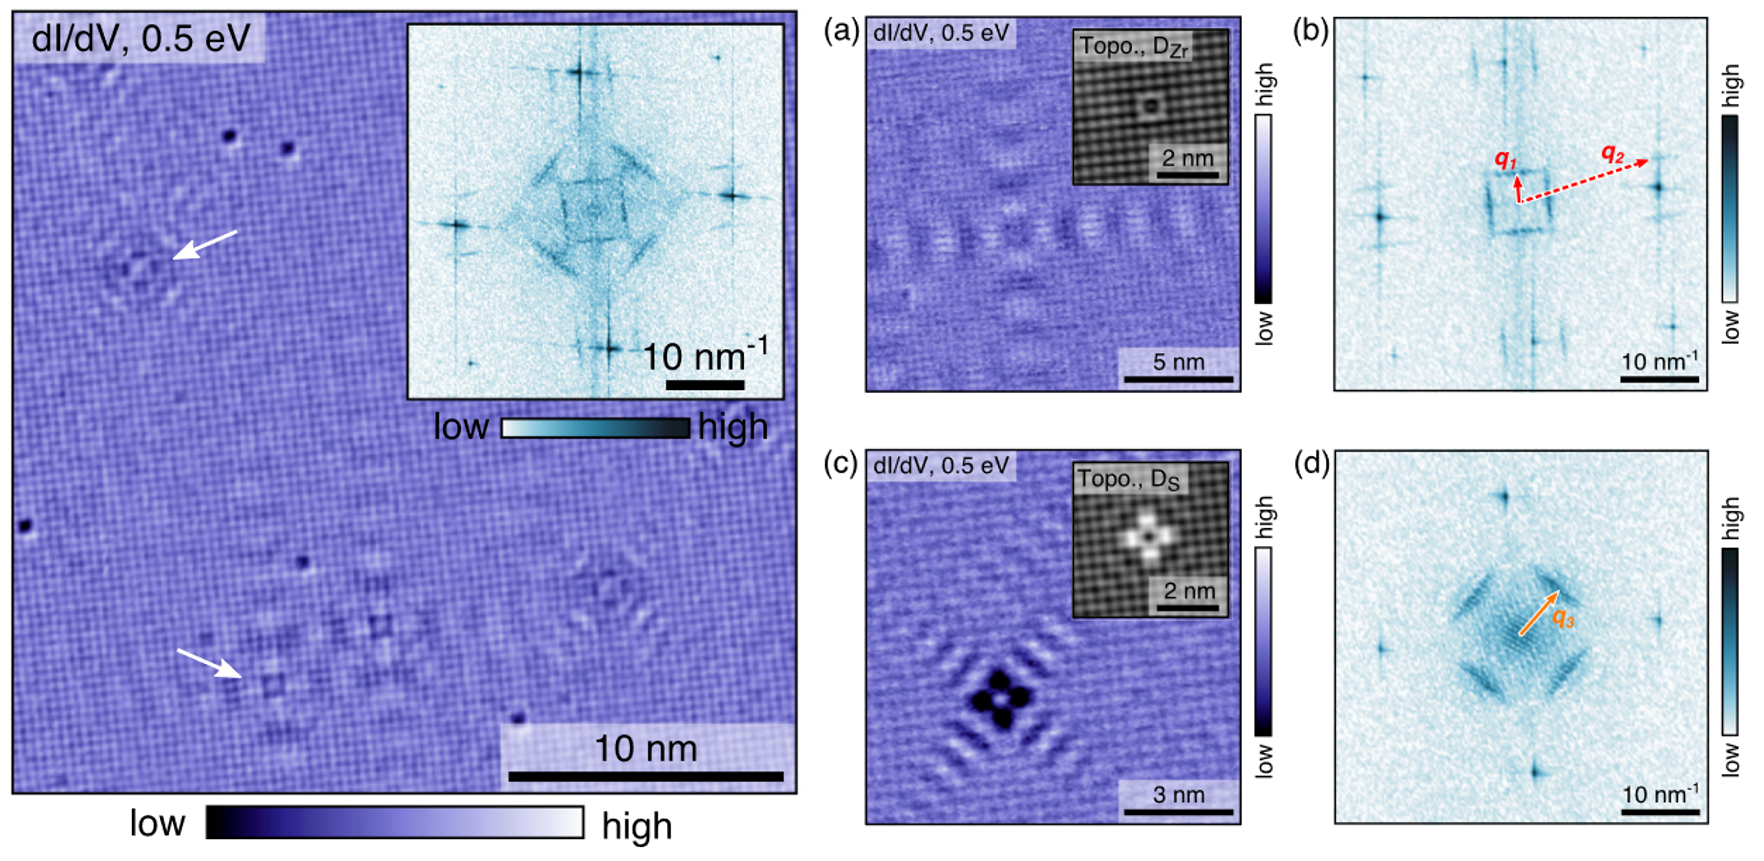
\includegraphics[width= \textwidth]{ZrSiS.png} 
	\centering
	\caption{Selective band scattering in ZrSiS. On the left, \ac{FT} of the whole grid map sees the band scattering. a)-d): The selective band scattering of different defects can be accessed by cropping around the individual defect QPI pattern and take the \ac{FT}/ However, due to the small spatial range of the cropped image, the q-space maps have limited resolution.}
	\label{fig:ch6_ZrSiS}
\end{figure}

\begin{figure}
	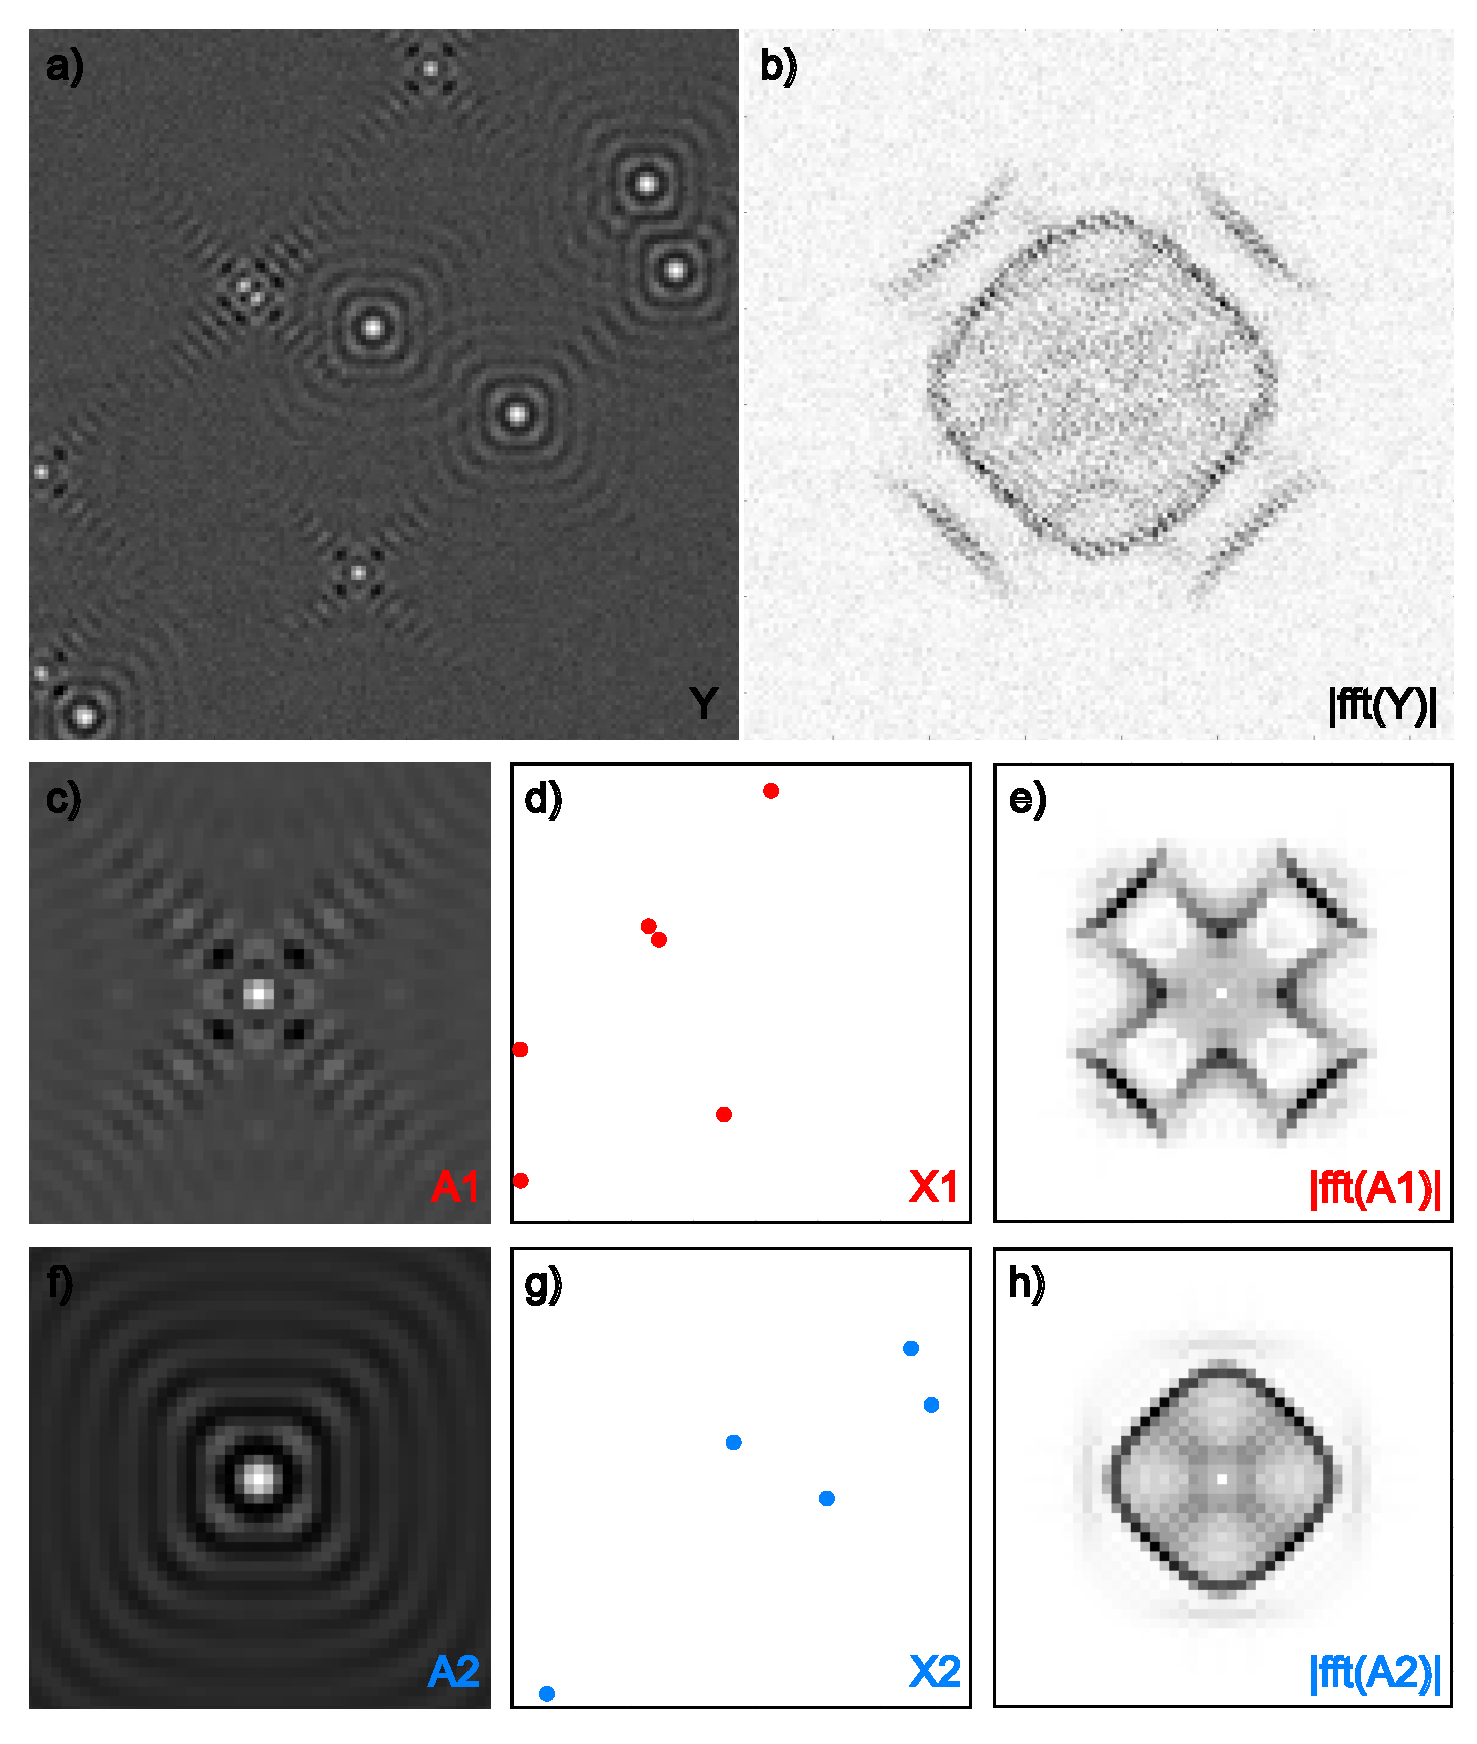
\includegraphics[width= \textwidth]{Ch6_demixing.pdf} 
	\centering
	\caption{Demixing as an inverse data generation process. Given the observation 
		$Y$ in (a), the goal is to reconstruct QPI patterns around individual impurities(kernels), as shown in (c) and (f). By applying a Fourier transform to each reconstructed kernel, we can isolate impurity-dependent scattering features, illustrated in (e) and (h).}
	\label{fig:ch6_demix}
\end{figure}

We now use our synthetic data to better illustrate the demixing problem. We simulate 2 \ac{QPI} patterns from 2 distinct defects with kernel choices A1 and A2 as shown in Fig. \ref{fig:ch6_demix} c) and d); We then define their activation maps X1 and X2 in d) and g). By summing up the convolutions between 2 kernels and their corresponding activation maps, we can obtain an observation Y in a). We express the above observation generation process as:

\begin{equation}
	Y = A1 * X1 + A2 * X2 + \beta, 
\end{equation}
where $\beta$ is the added noise determined by a pre-defined signal-to-noise ratio.

The demixing problem is the inverse of the observation generation process: given the observation Y, our goal is to reconstruct A1, A2. This means that in reciprocal space, rather than working with entangled and less informative data like (b), we can recover disentangled QPI patterns from individual defect types, as shown in (e) and (h), which are also free from speckle. Lastly, we extend the above formulation with multiple types of different defects, then at arbitrary energy $\omega$, we have: 

\begin{equation}
	\label{eq:demixing}
	Y_{\omega} = \sum_d ( A_{d,{\omega}} * X_d) + \beta. 
\end{equation} 



